
\noindent\rule{7in}{2.8pt}
\section{The Weak Interaction}
    
\begin{problem}{11.1}
Explain why the strong decay $\rho^0\to\pi^+\pi^-$ is observed, but the strong decay $\rho^0\to\pi^0\pi^0$ is not.
Hint : you will need to consider conservation of angular momentum, parity and the symmetry of the $\pi^0\pi^0$ wavefunction.
\end{problem}
\begin{solution}
d
\end{solution}

\noindent\rule{7in}{1.5pt}

%%%%%%%%%%%%%%%%%%%%%%%%%%%%%%%%%%%%%%%%%%%%%%%%%%%%%%%%%%%%%%%%%%%%%%%%%%%%%%%%%%%%%%%%%%%%%%%%%%%%%%%%%%%%%%%%%%%%%%%%%%%%%%%%%%%%%%%%

\begin{problem}{11.2}
When $\pi^-$ mesons are stopped in a deuterium target they can form a bound $(\pi^--D)$ state with zero orbital angular momentum, $l = 0$. The bound state decays by the strong interaction

\begin{align*}
    \pi^-D\to nn.
\end{align*}\\
By considering the possible spin and orbital angular momentum states of the nn system, and the required symmetry of the wavefunction, show that the pion has negative intrinsic parity.\\

Note : the deuteron has $J^P =1^+$ and the pion is a spin-0 particle.
\end{problem}
\begin{solution}
As the bound $\pi^- D$ state has $l=0$, the angular momentum conservation states that 

\begin{align*}
    J(D) + J(\pi^-) &= L(nn) + S(nn) \\
    1 + 0 &= L(nn) + S(nn)
\end{align*}\\
where $L(nn),S(nn)$ is the orbital, spin angular momentum of the $nn$ system. Upon the fact that neutrons are half-spin fermions, the available value of $S(nn)$ is either 0 or 1, which gives $L(nn)$ as 1 or 0 respectively. The $nn$ bound state which consists of two identical fermions, should have an antisymmetric overall wavefunction $\psi_{nn}=\psi^{\text{space}}_{nn}\times\psi^{\text{spin}}_{nn}$ according to the Pauli exclusion principle. $\psi^{\text{space}}_{nn}$ should be symmetric[?], thus to maintain the antisymmetry of $\psi_{nn}$, $\psi^{\text{spin}}_{nn}$ should be antisymmetric which only allows the pair of $S(nn)=0$ and $L(nn)=1$. Considering the parity conservation of the initial and the final state,

\begin{alignat}{2}
   &\quad P(\pi^-)\cdot P(D) \cdot (-1)^{l=0} &&= P(n)\cdot P(n) \cdot (-1)^{L(nn)} \nonumber \\[0.12in]
   &\implies P(\pi^-) \cdot (+1) \cdot (-1)^0 &&= (-1)^{L(nn)} \nonumber  \\[0.12in]
   &\implies P(\pi^-) = (-1)^{L(nn)=1}  &&= (-1)   \nonumber \qed
\end{alignat}
\end{solution}

\noindent\rule{7in}{1.5pt}

%%%%%%%%%%%%%%%%%%%%%%%%%%%%%%%%%%%%%%%%%%%%%%%%%%%%%%%%%%%%%%%%%%%%%%%%%%%%%%%%%%%%%%%%%%%%%%%%%%%%%%%%%%%%%%%%%%%%%%%%%%%%%%%%%%%%%%%%

\begin{problem}{11.3}
Classify the following quantities as either scalars (S), pseudoscalars (P), vectors (V) or axial-vectors (A):

\begin{enumerate}[label=(\alph*)]
    \item mechanical power, $P=\boldsymbol{F\cdot v}$;
    \item force, $\mathbf{F}$;
    \item torque, $\mathbf{G}=\boldsymbol{r\times F}$;
    \item vorticity, $\boldsymbol{\Omega}=\boldsymbol{\nabla \times v}$;
    \item magnetic flux, $\phi = \int \mathbf{B}\cdot \dif\mathbf{S}$;
    \item divergence of the electric field strength, $\boldsymbol{\nabla \cdot E}$.
\end{enumerate}
\end{problem}
\begin{solution}
    \begin{enumerate}[label=(\alph*)]
        \item mechanical power, $P=\boldsymbol{F\cdot v}$ : \textbf{scalar}
        \item force, $\mathbf{F}$ : \textbf{vector}
        \item torque, $\mathbf{G}=\boldsymbol{r\times F}$ : \textbf{axial vector}
        \item vorticity, $\boldsymbol{\Omega}=\boldsymbol{\nabla \times v}$ : \textbf{axial vector}
        \item magnetic flux, $\phi = \int \mathbf{B}\cdot \dif\mathbf{S}$ : \textbf{pseudoscalar} as $\mathbf{B}$ is an axial vector
        \item divergence of the electric field strength, $\boldsymbol{\nabla \cdot E}$ : \textbf{scalar}
    \end{enumerate}
\end{solution}

\noindent\rule{7in}{1.5pt}

%%%%%%%%%%%%%%%%%%%%%%%%%%%%%%%%%%%%%%%%%%%%%%%%%%%%%%%%%%%%%%%%%%%%%%%%%%%%%%%%%%%%%%%%%%%%%%%%%%%%%%%%%%%%%%%%%%%%%%%%%%%%%%%%%%%%%%%%

\begin{problem}{11.4}
In the annihilation process $e^+e^- \to qq$, the QED vector interaction leads to non-zero matrix elements only for the chiral combinations LR → LR, LR → RL, RL → RL, RL → LR. What are the corresponding allowed chiral combinations for S, P and S-P interactions?
\end{problem}
\begin{solution}
\begin{enumerate}[label=(\roman*)]
    \item $S$
    \item $P$
    \item $S-P$
\end{enumerate}
\end{solution}

\noindent\rule{7in}{1.5pt}

%%%%%%%%%%%%%%%%%%%%%%%%%%%%%%%%%%%%%%%%%%%%%%%%%%%%%%%%%%%%%%%%%%%%%%%%%%%%%%%%%%%%%%%%%%%%%%%%%%%%%%%%%%%%%%%%%%%%%%%%%%%%%%%%%%%%%%%%

\begin{problem}{11.5}
Consider the decay at rest $\tau^-\to\pi^-\nu_\tau$, where the spin of the tau is in the positive z-direction and the $\nu_\tau$ and $\pi^-$ travel in the $\pm z$-directions. Sketch the allowed spin configurations assuming that the form of the weak charged-current interaction is (i) V - A and (ii) V + A.
\end{problem}
\begin{solution}
    Note that for massless neutrinos, it is ok to regard helicity and chirality states with no big difference. 
    \begin{enumerate}[label=(\roman*)]
        \item $V-A$
        
        \begin{center}
            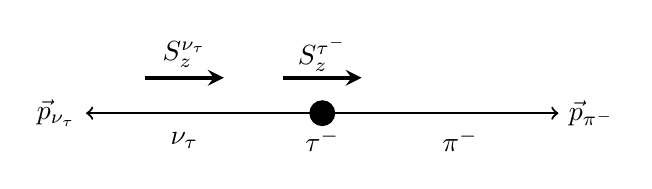
\begin{tikzpicture}
            
                \draw[thick, fill=black] (0,0) circle (0.15);
                \node at (0,-0.35) {$\tau^-$};
                \draw[thick, ->] (0,0) -- (3,0) node[right] {$\vec{p}_{\pi^-}$};
                \draw[thick, ->] (0,0) -- (-3,0) node[left] {$\vec{p}_{\nu_\tau}$};

                \draw[thick,  ->, >=stealth, line width=1.5pt] (-0.5,0.45) -- (0.5,0.45) ;
                \node at (0,0.75) {$S_z^{\tau^-}$};
                
                \draw[thick,  ->, >=stealth, line width=1.5pt] (-2.25,0.45) -- (-1.25,0.45) ;
                \node at (-1.75,0.75) {$S_z^{\nu_\tau}$};
                \node at (-1.75,-0.35) {$\nu_\tau$};
                \node at (1.75,-0.35) {$\pi^-$};

            \end{tikzpicture}
        \end{center}\vspace{0.1in}

        As seen in the textbook, the $V-A$ nature of the weak interaction projects out LH particles and RH antiparticles with the particles involved. The initial rest $\tau^-$ with its $z$ component spin aligned to $+z$ imposes that the final LH $\nu_\tau$ should also have $+z$ direction $z$ component spin, as pions are spin-0 particles. In order for such LH $\nu_\tau$ to have its spin aligned to $+z$, the momentum direction shall be in $-z$.  \vspace{0.1in}

        \item $V+A$
        
        \begin{center}
            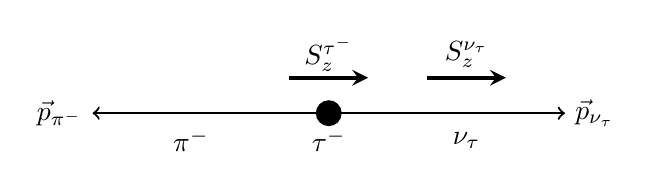
\begin{tikzpicture}
            
                \draw[thick, fill=black] (0,0) circle (0.15);
                \node at (0,-0.35) {$\tau^-$};
                \draw[thick, ->] (0,0) -- (3,0) node[right] {$\vec{p}_{\nu_\tau}$};
                \draw[thick, ->] (0,0) -- (-3,0) node[left] {$\vec{p}_{\pi^-}$};

                \draw[thick,  ->, >=stealth, line width=1.5pt] (-0.5,0.45) -- (0.5,0.45) ;
                \node at (0,0.75) {$S_z^{\tau^-}$};
                \draw[thick,  ->, >=stealth, line width=1.5pt] (1.25,0.45) -- (2.25,0.45) ;
                \node at (1.75,0.75) {$S_z^{\nu_\tau}$};

                \node at (-1.75,-0.35) {$\pi^-$};
                \node at (1.75,-0.35) {$\nu_\tau$};
                
            \end{tikzpicture}
        \end{center}\vspace{0.1in}
        
        Considering the interaction to have a form of $V+A$ which includes a $\sim (1+\gamma^5)$ term proportional to $P_R$, it will project out RH particles and LH antiparticles thus in this case the final $\nu_\tau$ should be right handed. Again as the angular moment should be conserves the outgoing RH $\nu_\tau$ shall have $+z$ directional $z$ component spin, thus the momentum shall be directed to the $+z$ direction.
    \end{enumerate}
\end{solution}

\noindent\rule{7in}{1.5pt}

%%%%%%%%%%%%%%%%%%%%%%%%%%%%%%%%%%%%%%%%%%%%%%%%%%%%%%%%%%%%%%%%%%%%%%%%%%%%%%%%%%%%%%%%%%%%%%%%%%%%%%%%%%%%%%%%%%%%%%%%%%%%%%%%%%%%%%%%

\begin{problem}{11.6}
Repeat the pion decay calculation for a pure scalar interaction and show that the predicted ratio of decay rates is

\begin{align*}
    \frac{\Gamma\left( \pi^- \to e^- \overbar{\nu}_e \right)}{\Gamma\left( \pi^- \to \mu^- \overbar{\nu}_\mu \right)} \approx 5.5 
\end{align*}\\
\end{problem}
\begin{solution}
If considering a pure scalar interaction, the matrix element can be approximated as, when using the same configuration of  $p_\pi = (m_\pi,0,0,0)$, $p_l = (E_l,0,0,p)$ and $p_{\overbar{\nu}} = (p,0,0,-p)$ 

\begin{align*}
    \mathcal{M}_{fi} = \left[gf_\pi m_\pi\right] \times \frac{1}{m^2} \times \left[ g \overbar{u}(p_l)v(p_{\overbar{\nu}})\right]  \sim  \overbar{u}(p_l)v(p_{\overbar{\nu}})
\end{align*}\\
where $g$ is the coupling constant of this scalar interaction and $m$ is the mass of the boson that mediates it. 
\end{solution}

\noindent\rule{7in}{1.5pt}

%%%%%%%%%%%%%%%%%%%%%%%%%%%%%%%%%%%%%%%%%%%%%%%%%%%%%%%%%%%%%%%%%%%%%%%%%%%%%%%%%%%%%%%%%%%%%%%%%%%%%%%%%%%%%%%%%%%%%%%%%%%%%%%%%%%%%%%%

\begin{problem}{11.7}
Predict the ratio of the $K^- \to e^- \nu_e$ and $K^- \to \mu^- \nu_\mu$ weak interaction decay rates and compare your answer to the measured value of

\begin{align*}
    \frac{\Gamma\left( K^- \to e^- \overbar{\nu}_e \right)}{\Gamma\left( K^- \to \mu^- \overbar{\nu}_\mu \right)} =   \left( 2.488\pm0.012 \right)\times 10^{-5}  
\end{align*}\\
\end{problem}
\begin{solution}

\end{solution}

\noindent\rule{7in}{1.5pt}

%%%%%%%%%%%%%%%%%%%%%%%%%%%%%%%%%%%%%%%%%%%%%%%%%%%%%%%%%%%%%%%%%%%%%%%%%%%%%%%%%%%%%%%%%%%%%%%%%%%%%%%%%%%%%%%%%%%%%%%%%%%%%%%%%%%%%%%%

\begin{problem}{11.8}
Charged kaons have several weak interaction decay modes, the largest of which are

\begin{align*}
    K^+\left( u\overbar{s} \right) \to \mu^+ \nu_\mu \comma K^+\to\pi^+\pi^0 \andtxt K^+\to\pi^+\pi^+\pi-
\end{align*}\\
\begin{enumerate}[label=(\alph*)]
    \item Draw the Feynman diagrams for these three weak decays.
    \item Using the measured branching ratio 
    
    \begin{align*}
        \text{Br}\left( K^+ \to \mu^+\nu_\mu \right) = 63.55 \pm 0.11 \%
    \end{align*}\\
    \textit{estimate} the lifetime of the charged Kaon.
\end{enumerate}\vspace{0.12in}
Note: charged pions decay almost 100\% of the time by the weak interaction $\pi^+\to\mu^+\nu_\mu$ and have a lifetime of $(2.6033 \pm 0.0005) \times 10^{-8} $s.
\end{problem}
\begin{solution}

\end{solution}

\noindent\rule{7in}{1.5pt}

%%%%%%%%%%%%%%%%%%%%%%%%%%%%%%%%%%%%%%%%%%%%%%%%%%%%%%%%%%%%%%%%%%%%%%%%%%%%%%%%%%%%%%%%%%%%%%%%%%%%%%%%%%%%%%%%%%%%%%%%%%%%%%%%%%%%%%%%

\begin{problem}{11.9}
From the prediction of (11.25) and the above measured value of the charged pion lifetime, obtain a value for $f_\pi$.
\end{problem}
\begin{solution}

\end{solution}

\noindent\rule{7in}{1.5pt}

%%%%%%%%%%%%%%%%%%%%%%%%%%%%%%%%%%%%%%%%%%%%%%%%%%%%%%%%%%%%%%%%%%%%%%%%%%%%%%%%%%%%%%%%%%%%%%%%%%%%%%%%%%%%%%%%%%%%%%%%%%%%%%%%%%%%%%%%

\begin{problem}{11.10}
Calculate the partial decay width for the decay $\tau^- \to \pi^-\nu_\tau$ in the following steps.

\begin{enumerate}[label=(\alph*)]
    \item Draw the Feynman diagram and show that the corresponding matrix element is
    
    \begin{align*}
        \mathcal{M} \approx \sqrt{2}G_F f_\pi \overbar{u}(p_\nu) \gamma^\mu \frac{1}{2}\left( 1-\gamma^5 \right) u(p_\tau)g_{\mu\nu}p_\pi^\nu
    \end{align*}\\
    \item Taking the $\tau^-$ spin to be in the $z-$direction and the four-momentum of the neutrino to be 
    
    \begin{align*}
        p_\nu = p^\ast \left( 1,\sin\theta,0,\cos\theta \right)
    \end{align*}\\
    show that the leptonic current is 

    \begin{align*}
        j^\mu = \sqrt{2m_\tau p^\ast } \left( -\sin\halftheta,-\cos\halftheta,-i\cos\halftheta,\sin\halftheta \right)
    \end{align*}\\
    Note that, for this configuration, the spinor for the $\tau^-$ can be taken to be $u_1$ for a particle at rest.

    \item Write down the four-momentum of the $\pi^-$ and show that
    
    \begin{align*}
        \big| \mathcal{M} \big|^2 = 4G_F^2 f_\pi^2 m_\tau^3 p^\ast \sin^2 \halftheta
    \end{align*}\\
    \item Hence show that 
    
    \begin{align*}
        \Gamma\left( \tau^- \to \pi^- \nu_\tau \right) = \frac{G_F^2 f_\pi^2}{16\pi} m_\tau^3 \left( \frac{m_\tau^2 - m_\pi^2}{m_\tau^2} \right)^2
    \end{align*}\\
    \item Using the value of $f_\pi$ obtained in the previous problem, find a numerical value for $\Gamma\left( \tau^- \to \pi^- \nu_\tau \right)$
    \item Given that the lifetime of the $\tau$ lepton is measured to be $\tau_\tau=\num{2.906e-13}$s, find an approximate value for the $\tau^- \to \pi^- \nu_\tau$ branching ratio.
\end{enumerate}
\end{problem}
\begin{solution}

\end{solution}

\noindent\rule{7in}{1.5pt}

%%%%%%%%%%%%%%%%%%%%%%%%%%%%%%%%%%%%%%%%%%%%%%%%%%%%%%%%%%%%%%%%%%%%%%%%%%%%%%%%%%%%%%%%%%%%%%%%%%%%%%%%%%%%%%%%%%%%%%%%%%%%%%%%%%%%%%%%
